\section{Unsupervised learning and clustering}

\begin{frame}{Supervised vs. unsupervised learning}
    \begin{itemize}
        \item Supervised: we observe predictors and a response, $\{(\mathbf{x}^{(i)}, y^{(i)})\}_{i=1}^{n}$, and learn $f$ such that $y \approx f(\mathbf{x})$
        \item Unsupervised: we observe only $\mathbf{x}^{(i)} \in \mathbb{R}^p$ for $i = 1, \dots, n$, collected in the $n \times p$ data matrix $\mathbf{X}$
        \item \dual{No response $y$: no ``correct answer'', no test error, no cross-validation of accuracy}{There is no response $y$, so there is no ``correct answer'' to compare against, no test error, and no cross-validation of prediction accuracy}
        \item The goal is to discover structure: subgroups of observations, relationships among variables, low-dimensional summaries
    \end{itemize}
\end{frame}

\begin{frame}{Clustering: the goal}
    \begin{itemize}
        \item Partition the $n$ observations into $K$ groups $C_1, \dots, C_K$ so that observations within a group are similar and observations in different groups are different
        \item Hard partition: $C_1 \cup \dots \cup C_K = \{1, \dots, n\}$ and $C_j \cap C_k = \emptyset$ for $j \neq k$
        \item Two ingredients: how to measure similarity (a distance) and how to search for a good partition (an algorithm)
        \item Examples: customer segmentation, grouping cell lines by gene expression, grouping districts by socio-economic indicators
    \end{itemize}
\end{frame}


\section{Distance and similarity measures}

\begin{frame}{Dissimilarity and similarity}
    \begin{itemize}
        \item A dissimilarity $d(\mathbf{x}^{(i)}, \mathbf{x}^{(l)}) \geq 0$ is small when two observations are alike; clustering only needs the $n \times n$ matrix of pairwise dissimilarities
        \item A distance (metric) also satisfies $d(\mathbf{x}, \mathbf{x}') = 0 \iff \mathbf{x} = \mathbf{x}'$, symmetry $d(\mathbf{x}, \mathbf{x}') = d(\mathbf{x}', \mathbf{x})$, and the triangle inequality
        \[
            d(\mathbf{x}, \mathbf{x}'') \leq d(\mathbf{x}, \mathbf{x}') + d(\mathbf{x}', \mathbf{x}'')
        \]
        \item A similarity $s$ is the opposite (large for alike observations); if $s \in [0, 1]$, then $d = 1 - s$ is a dissimilarity
        \item The choice of $d$ defines what ``similar'' means and can change the clusters more than the choice of algorithm
    \end{itemize}
\end{frame}

\begin{frame}{Minkowski distances}
    \begin{columns}[T]
        \begin{column}{0.62\textwidth}
            \begin{itemize}
                \item For $\mathbf{x}^{(i)}, \mathbf{x}^{(l)} \in \mathbb{R}^p$,
                \[
                    d_q(\mathbf{x}^{(i)}, \mathbf{x}^{(l)}) = \Bigl( \sum_{j=1}^{p} \bigl| x_j^{(i)} - x_j^{(l)} \bigr|^q \Bigr)^{1/q}
                \]
                \item $q = 2$ Euclidean: the default; squaring gives large gaps more weight
                \item $q = 1$ Manhattan: sum of absolute differences; less dominated by one large gap
                \item $q \to \infty$ Chebyshev: $\max_j |x_j^{(i)} - x_j^{(l)}|$; only the worst coordinate counts
            \end{itemize}
        \end{column}
        \begin{column}{0.36\textwidth}
            \centering
            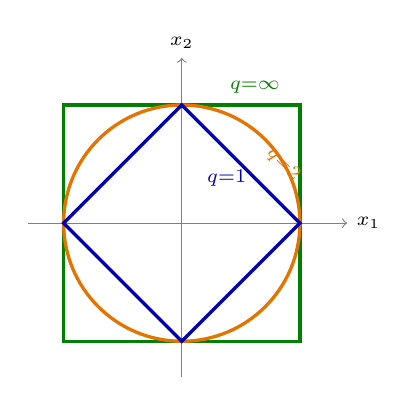
\begin{tikzpicture}[scale=1.5]
                \draw[->, gray] (-1.3, 0) -- (1.4, 0) node[right, black] {\scriptsize $x_1$};
                \draw[->, gray] (0, -1.3) -- (0, 1.4) node[above, black] {\scriptsize $x_2$};
                \draw[very thick, green!50!black] (-1, -1) rectangle (1, 1);
                \draw[very thick, orange!90!black] (0, 0) circle (1);
                \draw[very thick, blue!70!black] (1, 0) -- (0, 1) -- (-1, 0) -- (0, -1) -- cycle;
                \node[blue!70!black, font=\scriptsize] at (0.38, 0.38) {$q{=}1$};
                \node[orange!90!black, font=\scriptsize, rotate=-45] at (0.86, 0.5) {$q{=}2$};
                \node[green!50!black, font=\scriptsize] at (0.62, 1.15) {$q{=}\infty$};
            \end{tikzpicture}

            {\scriptsize Points at distance 1 from the origin}
        \end{column}
    \end{columns}
\end{frame}

\begin{frame}{Example data: USArrests}
    \begin{itemize}
        \item Violent crime in the 50 US states in 1973% ; available in R as \textttbg{USArrests}
        \item No response and no group labels: a natural setting for unsupervised learning
        \item Variables are on different scales: three arrest rates per 100{,}000 residents and one percentage
    \end{itemize}
    \svspace{0.5em}
    \centering
    \footnotesize
    \begin{tabular}{@{}l l r r@{}}
        \toprule
        Variable & Description & Mean & SD \\
        \midrule
        Murder & murder arrests per 100{,}000 residents & 7.79 & 4.36 \\
        Assault & assault arrests per 100{,}000 residents & 170.76 & 83.34 \\
        UrbanPop & percent of the population living in urban areas & 65.54 & 14.47 \\
        Rape & rape arrests per 100{,}000 residents & 21.23 & 9.37 \\
        \bottomrule
    \end{tabular}

    \svspace{0.5em}
    {\scriptsize Sources: World Almanac and Book of Facts 1975 (arrests); Statistical Abstracts of the United States 1975 (urban population)}
\end{frame}

\begin{frame}{Scale matters: standardize first}
    \begin{columns}[T]
        \begin{column}{0.54\textwidth}
            \begin{itemize}
                \item A variable measured on a large scale dominates the sum of squared (or absolute) differences
                \item Standardize each variable before computing distances:
                \[
                    z_j^{(i)} = \frac{x_j^{(i)} - \bar{x}_j}{s_j}
                \]
                \item Exception: variables already on a common, meaningful scale (e.g. counts of the same item)
            \end{itemize}
        \end{column}
        \begin{column}{0.44\textwidth}
            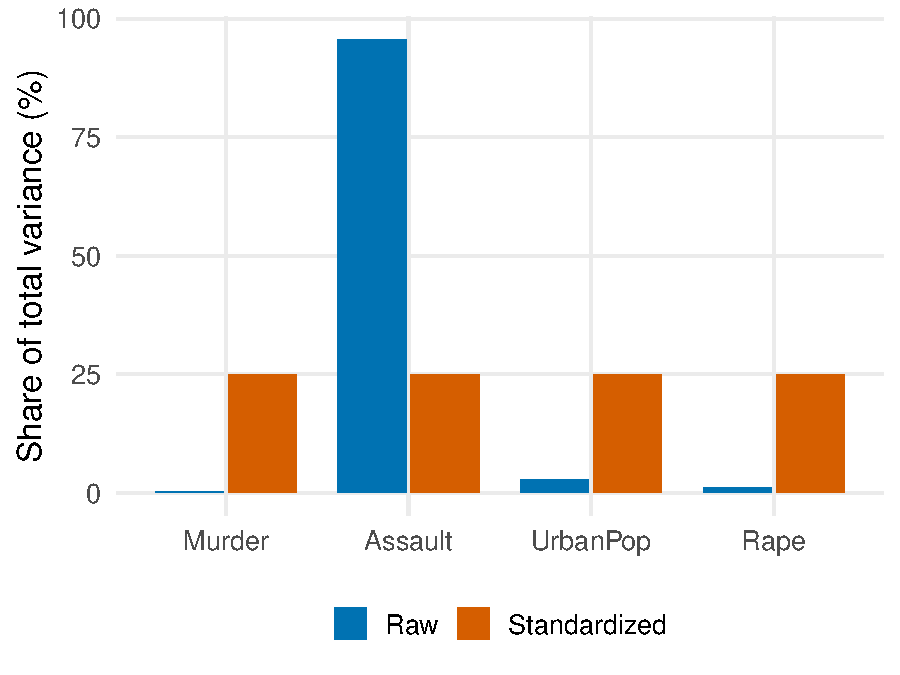
\includegraphics[width=\textwidth, height=0.5\textheight, keepaspectratio]{figures/fig_usarrests_variance.pdf}

            {\scriptsize USArrests: share of total variance}
        \end{column}
    \end{columns}
\end{frame}

\begin{frame}{Mahalanobis distance}
    \begin{itemize}
        \item Let $\mathbf{S}$ be the sample covariance matrix of the variables. Then
        \[
            d_M(\mathbf{x}^{(i)}, \mathbf{x}^{(l)}) = \sqrt{(\mathbf{x}^{(i)} - \mathbf{x}^{(l)})^\top \mathbf{S}^{-1} (\mathbf{x}^{(i)} - \mathbf{x}^{(l)})}
        \]
        \item Rescales each variable and accounts for correlation between variables; equals Euclidean distance if $\mathbf{S} = \mathbf{I}$
        \item Use when variables are strongly correlated, so that Euclidean distance counts the same information several times
        \item Needs an invertible $\mathbf{S}$ (so $n > p$ and no exact collinearity), and $\mathbf{S}$ is estimated from all data, not within clusters
    \end{itemize}
\end{frame}

\begin{frame}{Correlation-based distance and cosine similarity}
    \begin{itemize}
        \item Correlation between the profiles of observations $i$ and $l$ across the $p$ variables, where $\bar{x}^{(i)}$ is the mean of observation $i$ over its $p$ variables:
        \[
            r_{il} = \frac{\sum_{j} (x_j^{(i)} - \bar{x}^{(i)})(x_j^{(l)} - \bar{x}^{(l)})}{\sqrt{\sum_{j} (x_j^{(i)} - \bar{x}^{(i)})^2} \sqrt{\sum_{j} (x_j^{(l)} - \bar{x}^{(l)})^2}}, \qquad d_{\text{cor}}(i, l) = 1 - r_{il}
        \]
        \item Cosine similarity is the same quantity without centering:
        \[
            \cos\theta_{il} = \frac{\mathbf{x}^{(i)\top} \mathbf{x}^{(l)}}{\lVert \mathbf{x}^{(i)} \rVert \, \lVert \mathbf{x}^{(l)} \rVert}
        \]
    \end{itemize}
\end{frame}

\begin{frame}{When shape matters more than level}
    \begin{columns}[T]
        \begin{column}{0.5\textwidth}
            \begin{itemize}
                \item Observations 1 and 3 have the same profile shape at different levels; observation 2 is flat
                \item Euclidean distance calls 1 and 2 close and 1 and 3 far apart; correlation distance says the opposite
                \item Use it when profile shape matters, not level (gene expression, shopping baskets, text); variables must be on comparable scales
            \end{itemize}
        \end{column}
        \begin{column}{0.48\textwidth}
            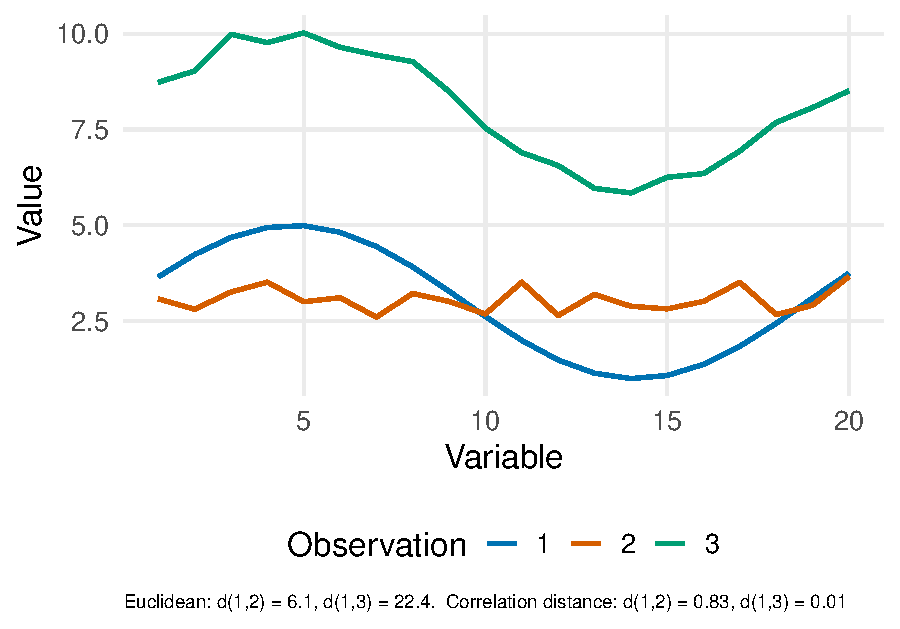
\includegraphics[width=\textwidth, height=0.5\textheight, keepaspectratio]{figures/fig_corr_distance.pdf}

            {\scriptsize Simulated: 3 observations on 20 variables. 1 is a sine curve, 3 is observation 1 shifted up by 5, 2 is flat noise around 3.}
        \end{column}
    \end{columns}
\end{frame}

\begin{frame}{Binary and categorical variables}
    \begin{itemize}
        \item For two binary vectors, count the variables where they are $(1,1)$, $(1,0)$, $(0,1)$ and $(0,0)$: $n_{11}$, $n_{10}$, $n_{01}$, $n_{00}$, with $p = n_{11} + n_{10} + n_{01} + n_{00}$
        \item Simple matching: $s = \dfrac{n_{11} + n_{00}}{p}$
            \begin{itemize}
                \item use when $0$ and $1$ are equally informative (symmetric), e.g. sex, urban/rural
            \end{itemize}
        \item Jaccard: $s = \dfrac{n_{11}}{n_{11} + n_{10} + n_{01}}$
            \begin{itemize}
                \item use when only presence is informative, e.g. rare symptoms, species present, items purchased
            \end{itemize}
        \item Categorical variables with more than two levels: $s$ is the fraction of variables on which the two observations agree; distance is $d = 1 - s$
    \end{itemize}
\end{frame}

\begin{frame}{Mixed data: Gower dissimilarity}
    \begin{itemize}
        \item Survey data typically mix continuous, ordinal and categorical variables; Gower combines per-variable similarities
        \[
            s_{il} = \frac{\sum_{j=1}^{p} w_j^{il} \, s_j^{il}}{\sum_{j=1}^{p} w_j^{il}}, \qquad d_{il} = 1 - s_{il}
        \]
        \item Continuous: $s_j^{il} = 1 - |x_j^{(i)} - x_j^{(l)}| / R_j$, where $R_j$ is the range of variable $j$
        \item Categorical: $s_j^{il} = 1$ if $x_j^{(i)} = x_j^{(l)}$ and $0$ otherwise; ordinal variables can use their ranks
        \item $w_j^{il} = 0$ if variable $j$ is missing for $i$ or $l$, else $1$
        % \item In R: \textttbg{cluster::daisy(x, metric = "gower")}
    \end{itemize}
\end{frame}

\begin{frame}{Choosing a dissimilarity: summary}
    \centering
    \footnotesize
    \begin{tabular}{@{}l l p{6.2cm}@{}}
        \toprule
        Measure & Variables & Use when \\
        \midrule
        Euclidean & continuous & default; variables standardized, compact groups \\
        Manhattan & continuous, counts & robustness to a single large difference \\
        Mahalanobis & continuous & strongly correlated variables, $n > p$ \\
        Correlation, cosine & continuous & profile shape matters more than level \\
        Matching & binary, categorical & $0$ and $1$ equally informative \\
        Jaccard & binary & only presence is informative \\
        Gower & mixed & continuous, ordinal and categorical variables together \\
        \bottomrule
    \end{tabular}
\end{frame}


\section{K-means clustering}

\begin{frame}{K-means: the objective}
    \begin{itemize}
        \item $K$ is the number of clusters, chosen in advance; each cluster $C_k$ is summarized by its mean (centroid), hence ``K-means'':
        \[
            \bar{\mathbf{x}}_k = \frac{1}{|C_k|} \sum_{i \in C_k} \mathbf{x}^{(i)}
        \]
        \item Find the partition that minimizes the total within-cluster sum of squares
        \[
            \min_{C_1, \dots, C_K} \; \sum_{k=1}^{K} \sum_{i \in C_k} \bigl\lVert \mathbf{x}^{(i)} - \bar{\mathbf{x}}_k \bigr\rVert^2
        \]
        \item Equivalent (up to a factor of 2) to making pairwise squared distances within each cluster small: $\frac{1}{|C_k|} \sum_{i, l \in C_k} \lVert \mathbf{x}^{(i)} - \mathbf{x}^{(l)} \rVert^2$
    \end{itemize}
\end{frame}

\begin{frame}{K-means: the algorithm}
    There are almost $K^n / K!$ partitions: exhaustive search is impossible, so we need an algorithm.
    \begin{enumerate}
        \item Randomly assign each observation to one of $K$ clusters
        \item Repeat until the assignments stop changing:
            \begin{enumerate}[(a)]
                \item compute the centroid $\bar{\mathbf{x}}_k$ of each cluster
                \item assign each observation to the cluster with the closest centroid (Euclidean distance)
            \end{enumerate}
    \end{enumerate}
    \svspace{1em}
    \begin{itemize}
        \item This procedure is known as Lloyd's algorithm
        \item Each pass is cheap, $O(npK)$, so K-means scales to large $n$
        % \item In R: \textttbg{kmeans(x, centers = K, nstart = 25)}
    \end{itemize}
\end{frame}

\begin{frame}{Why the algorithm decreases the objective}
    \begin{itemize}
        \item For any cluster $C$ and any point $\mathbf{m}$,
        \[
            \sum_{i \in C} \lVert \mathbf{x}^{(i)} - \mathbf{m} \rVert^2 = \sum_{i \in C} \lVert \mathbf{x}^{(i)} - \bar{\mathbf{x}}_C \rVert^2 + |C| \, \lVert \bar{\mathbf{x}}_C - \mathbf{m} \rVert^2
        \]
        \item Step (a): the centroid is the best center for its cluster, so the objective cannot increase
        \item Step (b): moving an observation to its nearest centroid reduces its squared distance, so the objective cannot increase
        \item The objective is bounded below and there are finitely many partitions, so the algorithm converges, but only to a local optimum: a partition that neither step can improve, which need not be the best partition overall
    \end{itemize}
\end{frame}

\begin{frame}{Example data: simulated clusters}
    \begin{itemize}
        \item The K-means examples, and some later ones, use simulated data with two variables, $x_1$ and $x_2$, so the true groups are known and can be plotted
        \item Each group is a round normal cloud: both coordinates are drawn independently from $N(\mu, \sigma^2)$ around the group's center
        \item Three-cluster data (K-means iterations): 3 groups of 50 observations, centers $(0, 0)$, $(4, 3)$ and $(-0.5, 4.5)$, $\sigma = 0.9$
        \item Four-cluster data (multiple starts, and later choosing $K$): 4 groups of 60 observations at the corners of a square, $(0, 0)$, $(4, 0)$, $(0, 4)$ and $(4, 4)$, $\sigma = 0.8$
        \item Smaller simulated sets used for single examples are described on the slides where they appear
    \end{itemize}
\end{frame}

\begin{frame}{K-means in action}
    \centering
    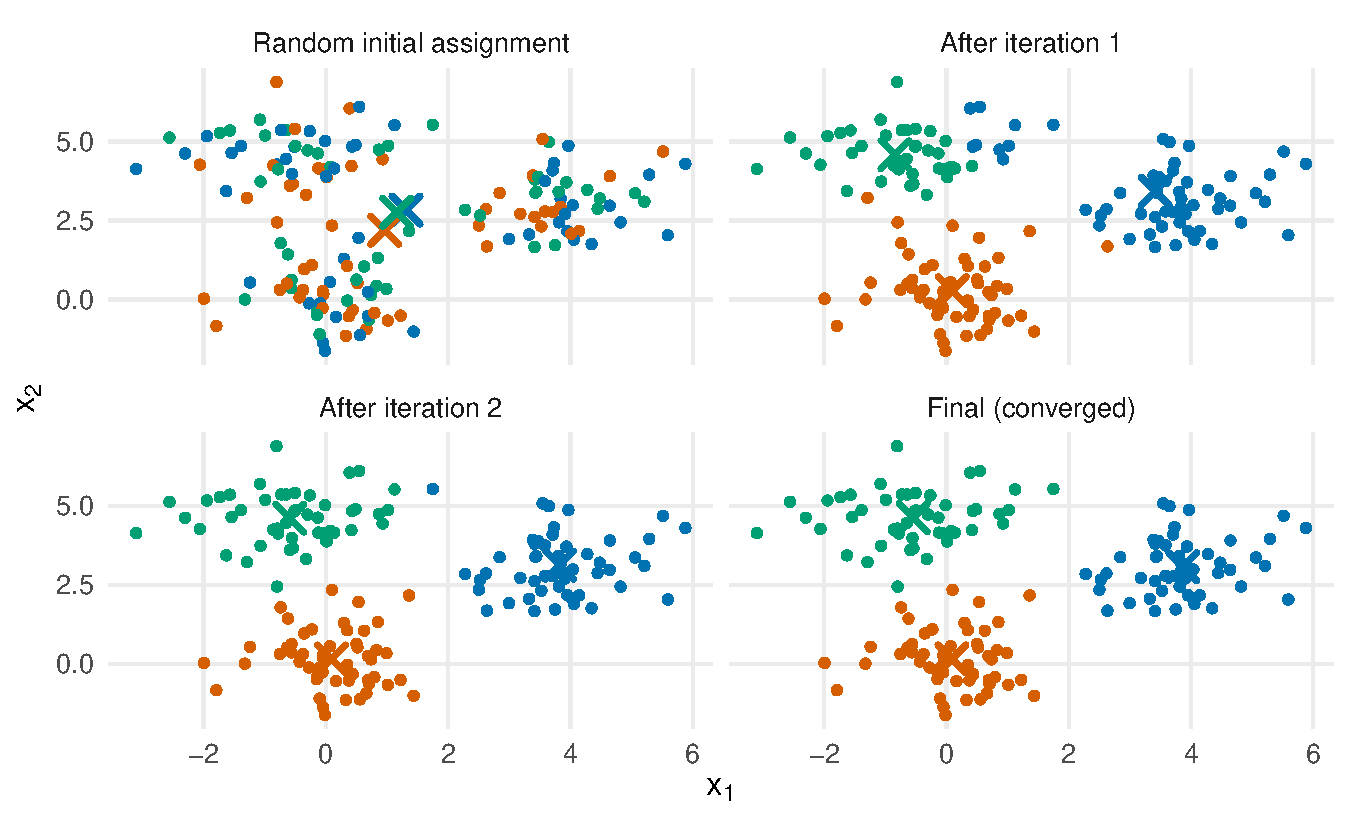
\includegraphics[width=\textwidth, height=0.72\textheight, keepaspectratio]{figures/fig_kmeans_iter.pdf}

    {\scriptsize Three-cluster simulated data, $K = 3$. Crosses mark the centroids.}
\end{frame}

\begin{frame}{Local optima and multiple starts}
    \centering
    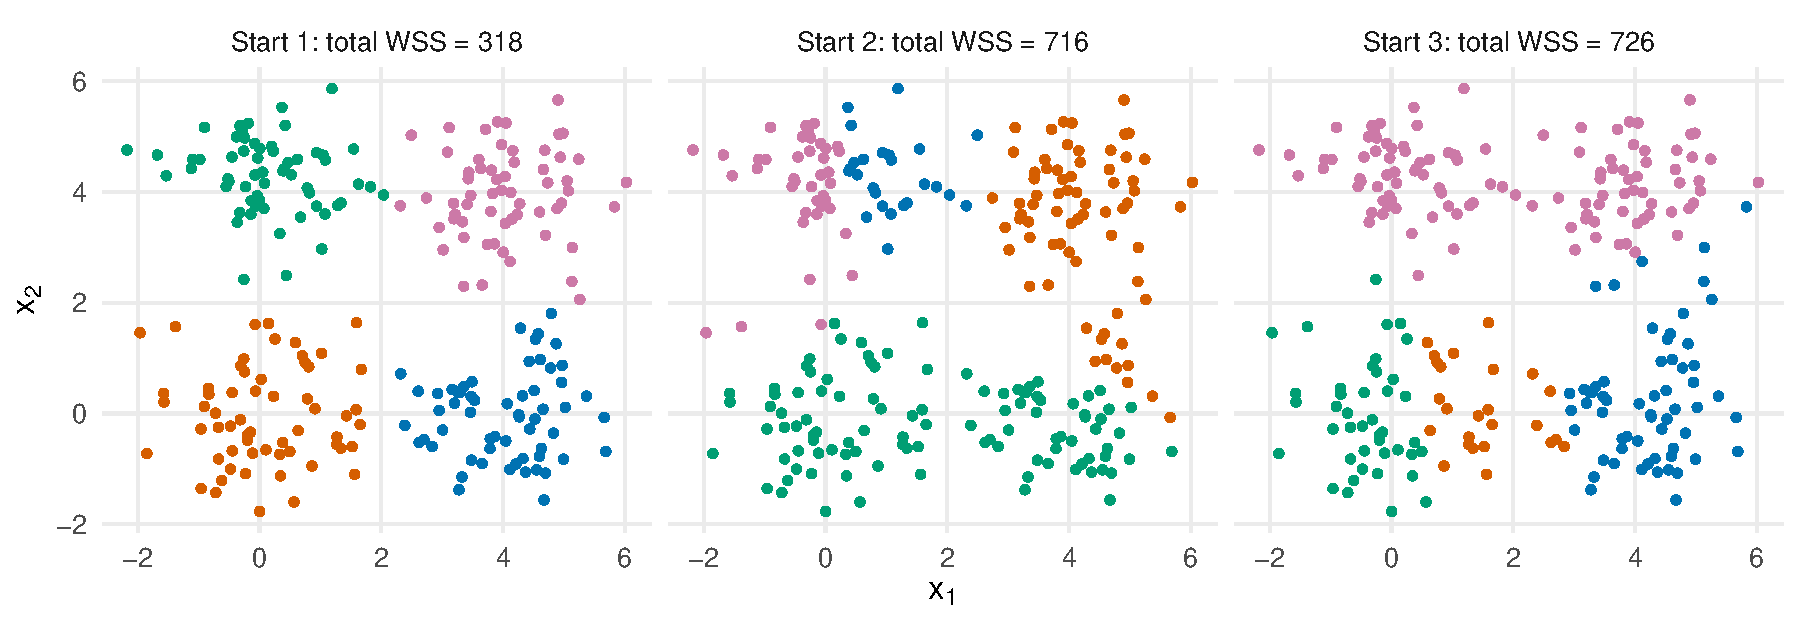
\includegraphics[width=\textwidth, height=0.32\textheight, keepaspectratio]{figures/fig_kmeans_starts.pdf}
    \begin{itemize}
        \item Four-cluster data, $K = 4$, three single starts: the solution depends on the random initial assignment, and different starts can end in different local optima
        \item Run the algorithm from many random starts and keep the solution with the smallest objective% (\textttbg{nstart})
        \item Smarter initialization, k-means++: choose the initial centroids one at a time, each new one more likely to be a point far from those already chosen
    \end{itemize}
\end{frame}

\begin{frame}{Choosing $K$ and assigning new observations}
    \begin{itemize}
        \item $K$ must be specified before running the algorithm; the evaluation section covers how to choose it
        \item The objective always decreases as $K$ grows, so it cannot be minimized over $K$
        \item A new observation $\mathbf{x}^\ast$ is assigned to the nearest centroid:
        \[
            \hat{k}^\ast = \arg\min_{k} \bigl\lVert \mathbf{x}^\ast - \bar{\mathbf{x}}_k \bigr\rVert
        \]
        \item Standardize $\mathbf{x}^\ast$ using the means and standard deviations of the data used to fit the clusters
    \end{itemize}
\end{frame}

\begin{frame}{Strengths and limitations of K-means}
    \centering
    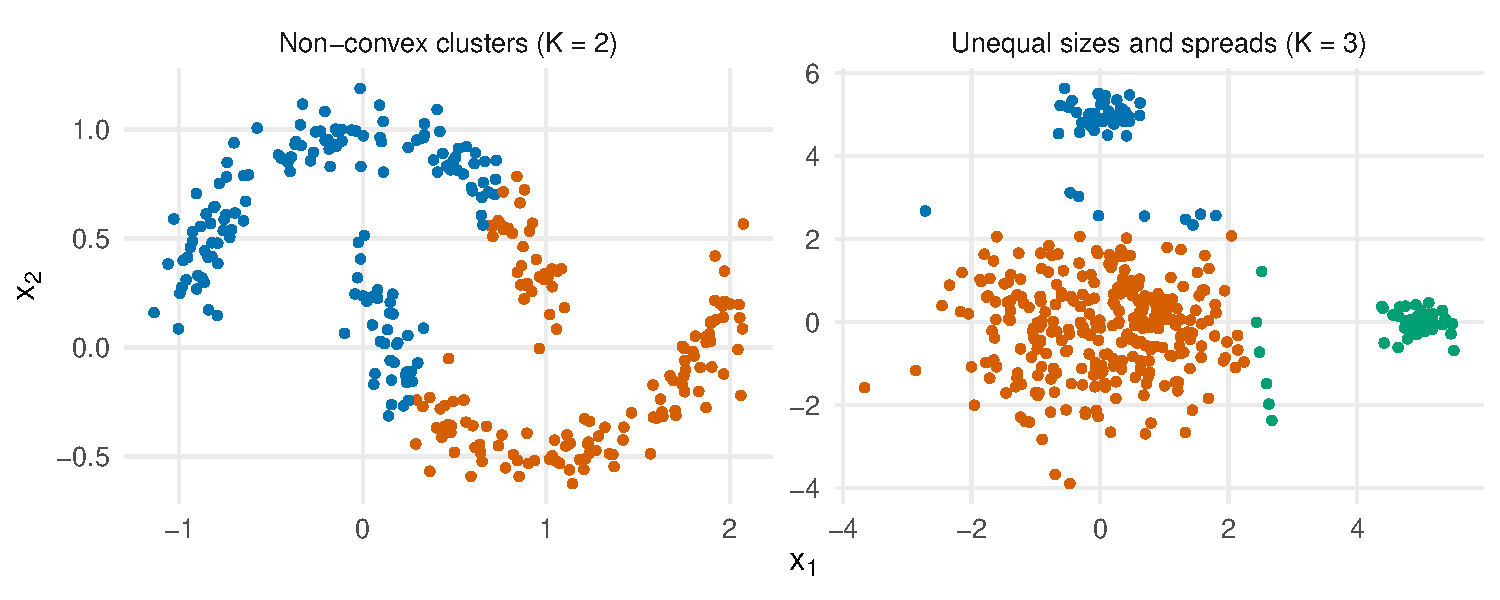
\includegraphics[width=\textwidth, height=0.28\textheight, keepaspectratio]{figures/fig_kmeans_limits.pdf}

    {\scriptsize Simulated. Left: two interleaved half-moons of 150 points each. Right: one large, spread-out group (300 points, $\sigma = 1.2$) and two small, tight groups (40 points each, $\sigma = 0.3$).}
    \begin{itemize}
        \item Strengths: simple, fast, works well for compact, roughly spherical clusters of similar size
        \item Limitations: non-convex shapes (such as the half-moons), very unequal sizes or spreads, and outliers (centroids are means) can give poor clusters
        \item Also requires $K$, depends on the starting point, and assigns every observation to a cluster
    \end{itemize}
\end{frame}


\section{Hierarchical clustering}

\begin{frame}{Hierarchical clustering: the idea}
    \begin{itemize}
        \item K-means needs $K$ in advance; hierarchical clustering does not
        \item It builds a tree of nested clusters, the dendrogram, from which any number of clusters can be read off
        \item Agglomerative (bottom-up) is the most common: start with $n$ singleton clusters and repeatedly fuse the two closest clusters
        \item The name comes from ``agglomerate'', to gather into a mass: clusters are built up by merging smaller ones
        \item Divisive (top-down) does the reverse: start with all $n$ observations in one cluster and repeatedly split
        \item Needs a dissimilarity between observations and a rule for the dissimilarity between clusters (the linkage)
    \end{itemize}
\end{frame}

\begin{frame}{Agglomerative algorithm}
    \begin{enumerate}
        \item Start with $n$ clusters, one per observation, and compute all $\binom{n}{2}$ pairwise dissimilarities
        \item For $i = n, n-1, \dots, 2$:
            \begin{enumerate}[(a)]
                \item find the pair among the $i$ clusters with the smallest inter-cluster dissimilarity and fuse them; the dissimilarity is the height of the fusion in the dendrogram
                \item recompute the inter-cluster dissimilarities among the remaining $i - 1$ clusters
            \end{enumerate}
    \end{enumerate}
    % \svspace{1em}
    % \begin{itemize}
        % \item In R: \textttbg{hclust(dist(x), method = "complete")}
    % \end{itemize}
\end{frame}

\begin{frame}{Divisive clustering}
    \begin{itemize}
        \item Top-down: start with all $n$ observations in one cluster and repeatedly split a cluster in two, until every observation is on its own
        \item A cluster of $m$ observations can be split in two in $2^{m-1} - 1$ ways, too many to check, so methods use heuristics:
            \begin{itemize}
                \item DIANA: split the cluster with the largest diameter (largest dissimilarity between two of its members); the member farthest on average from the rest starts a splinter group, and members closer on average to the splinter group move over
                \item Bisecting K-means: split a cluster with K-means, $K = 2$
            \end{itemize}
        \item In DIANA the height of a split is the diameter of the cluster split, so the result is again a dendrogram
        \item Settles the large clusters first, so it can do better when only a few big groups matter; less common in practice than agglomerative
    \end{itemize}
\end{frame}

\begin{frame}{Linkage: dissimilarity between clusters}
    Let $A$ and $B$ be two clusters and $d_{il} = d(\mathbf{x}^{(i)}, \mathbf{x}^{(l)})$.
    \begin{itemize}
        \item Complete: $d(A, B) = \max_{i \in A,\, l \in B} d_{il}$
        \item Single: $d(A, B) = \min_{i \in A,\, l \in B} d_{il}$
        \item Average: $d(A, B) = \dfrac{1}{|A|\,|B|} \sum_{i \in A} \sum_{l \in B} d_{il}$
        \item Centroid: $d(A, B) = d(\bar{\mathbf{x}}_A, \bar{\mathbf{x}}_B)$, the dissimilarity between the two cluster centroids
        \item Ward: fuse the pair of clusters whose merger increases the total within-cluster sum of squares the least (the K-means objective)
    \end{itemize}
\end{frame}

\begin{frame}{Reading a dendrogram}
    \centering
    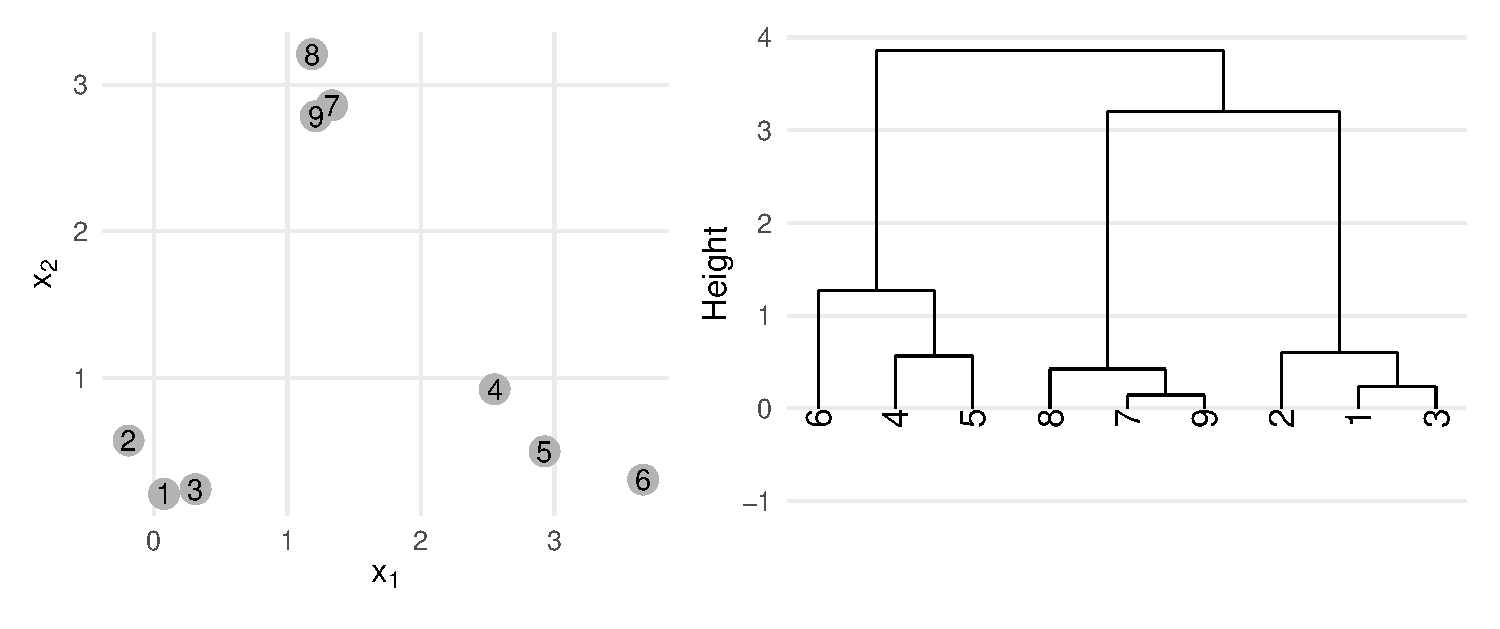
\includegraphics[width=\textwidth, height=0.42\textheight, keepaspectratio]{figures/fig_dendro_reading.pdf}

    {\scriptsize Simulated: 9 points in three groups of three; Euclidean distance, complete linkage}
    \begin{itemize}
        \item Each leaf is an observation; the height of a fusion is the dissimilarity at which the two clusters joined
        \item Similarity of two observations is judged by the height where they first fuse, not by how close their leaves are horizontally
        \item Cutting the tree at a height gives a partition into clusters
    \end{itemize}
\end{frame}

\begin{frame}{Effect of linkage}
    \centering
    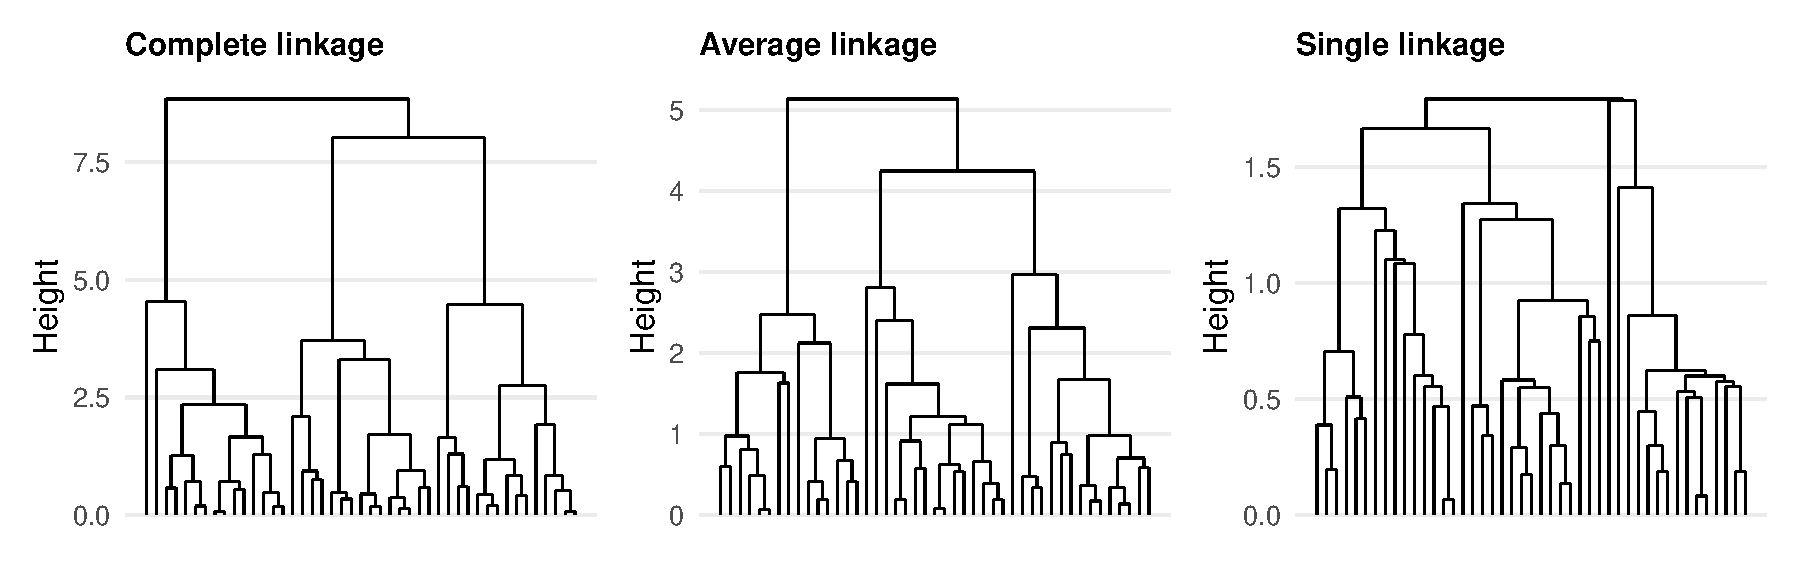
\includegraphics[width=\textwidth, height=0.4\textheight, keepaspectratio]{figures/fig_linkage_compare.pdf}

    {\scriptsize Simulated: 45 points in three groups of 15 ($\sigma = 1$); Euclidean distance}
    \begin{itemize}
        \item Complete and average: compact, fairly balanced clusters; complete is the usual default
        \item Single: chaining, where clusters grow by adding one point at a time; useful for elongated groups, but gives trailing, unbalanced trees
        \item Centroid: popular in genomics, but can produce inversions (a fusion lower than an earlier one)
    \end{itemize}
\end{frame}

\begin{frame}{Cutting the tree}
    \begin{itemize}
        \item Choose the number of clusters $K$ or a height $h$ at which to cut% (\textttbg{cutree(hc, k = K)})
        \item A large gap between successive fusion heights suggests a natural place to cut, but this is a judgment call
        \item Clusters are nested: those for $K = 2$ are merged clusters of $K = 3$
        \item Nesting can be unrealistic: a population split by sex and by nationality does not form a single hierarchy
    \end{itemize}
\end{frame}

\begin{frame}{Divisive vs. agglomerative}
    \centering
    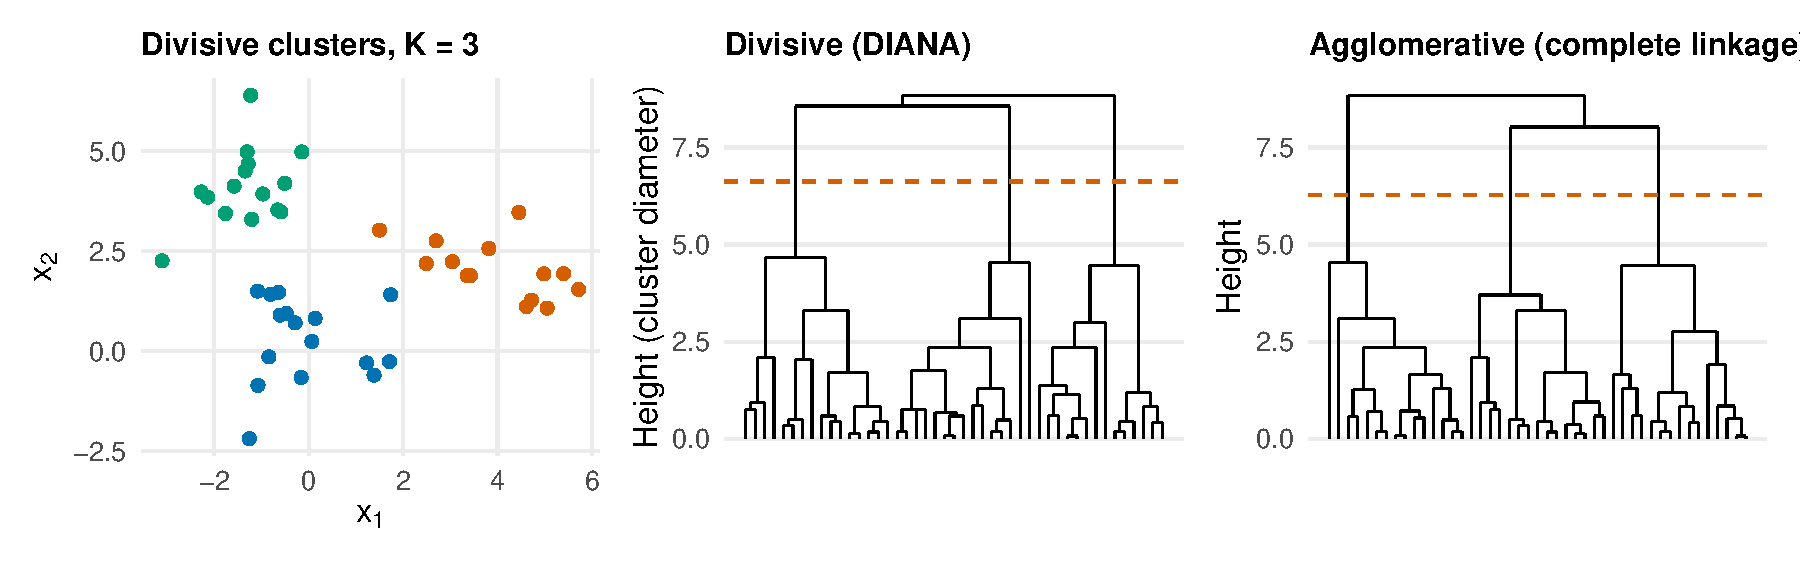
\includegraphics[width=\textwidth, height=0.4\textheight, keepaspectratio]{figures/fig_divisive.pdf}

    {\scriptsize Same 45 simulated points as the linkage comparison; Euclidean distance. Dashed lines cut each tree into $K = 3$ clusters.}
    \begin{itemize}
        \item Left: the three clusters from the divisive (DIANA) tree; cutting the complete-linkage tree gives the same clusters except for one point
        \item Both trees are read the same way; in the divisive tree the height of a split is the diameter of the cluster being split
    \end{itemize}
\end{frame}

\begin{frame}{Effect of scaling on the clusters}
    \centering
    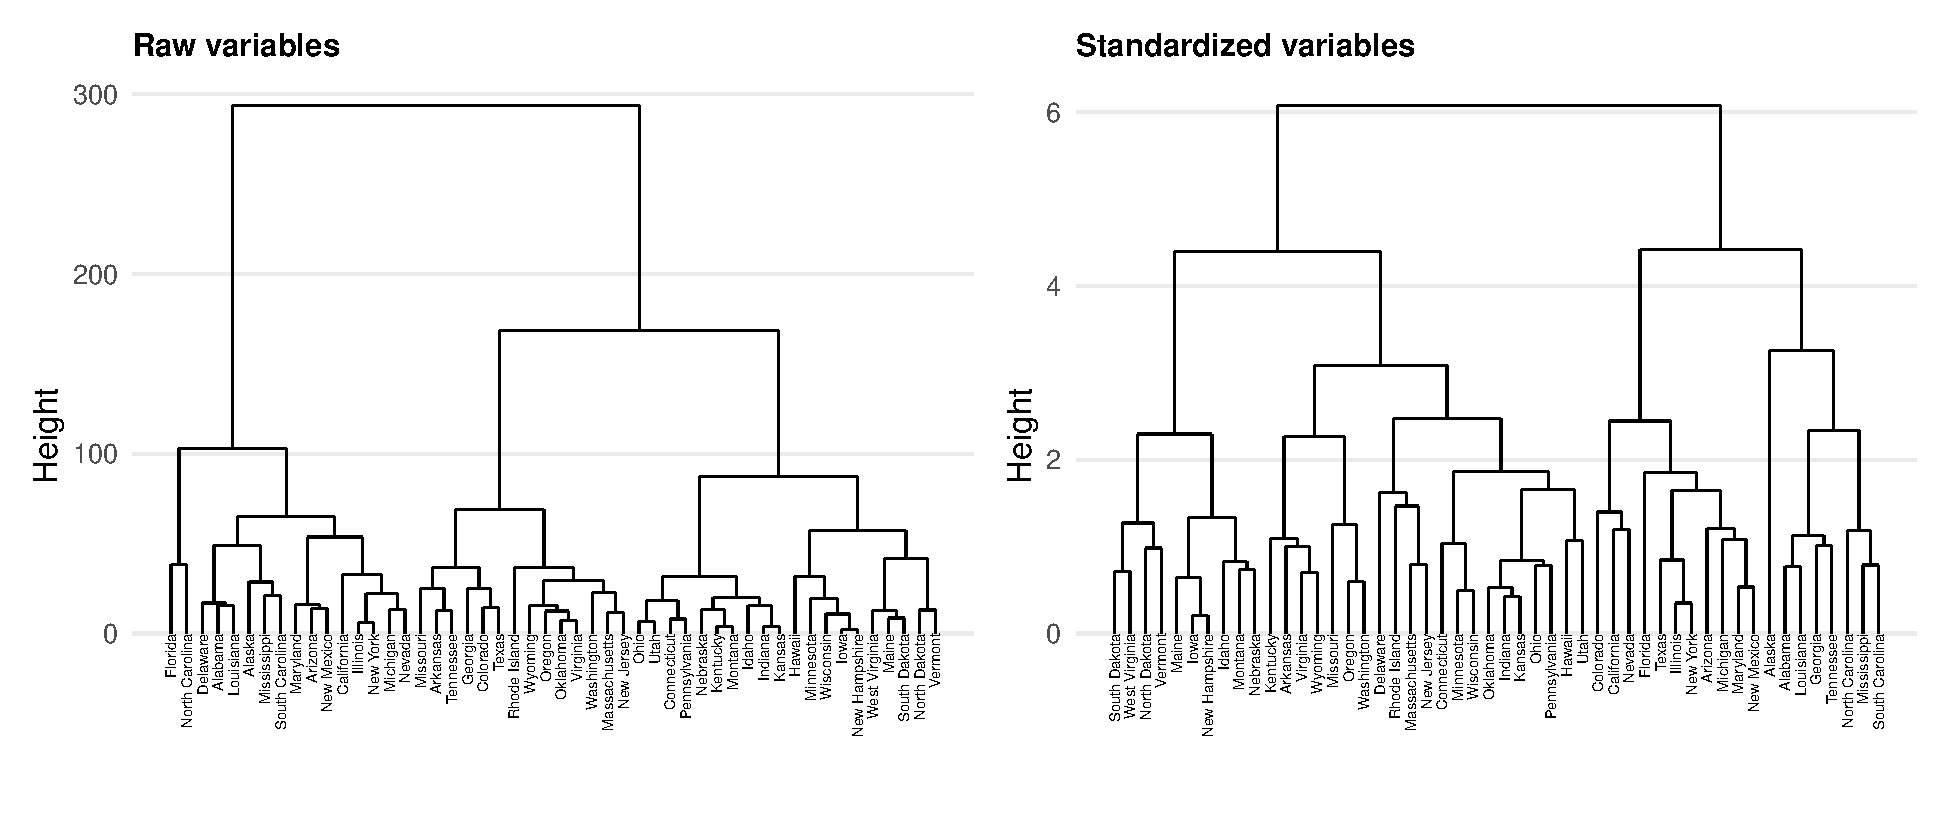
\includegraphics[width=\textwidth, height=0.5\textheight, keepaspectratio]{figures/fig_usarrests_scale_dendro.pdf}
    \begin{itemize}
        \item USArrests, Euclidean distance, complete linkage: on raw data the tree is driven almost entirely by Assault, the variable with by far the largest variance
        \item After standardizing, all four variables contribute and the grouping of states changes
    \end{itemize}
\end{frame}

\begin{frame}{Example data: NCI60}
    \begin{itemize}
        \item Gene expression for 64 human cancer cell lines (tumor cells grown in the laboratory) from the US National Cancer Institute's NCI-60 panel, measured with microarrays, which record the activity of thousands of genes at once (Ross et al., 2000)% ; in R: \textttbg{ISLR2::NCI60}
        \item $p = 6{,}830$ genes per cell line, far more variables than observations ($p \gg n$), so Mahalanobis distance cannot be used; each gene is standardized before computing distances
        \item Each cell line carries a cancer-type label (14 labels):
            \begin{itemize}
                \item breast 7, CNS 5, colon 7, leukemia 6, melanoma 8, non-small cell lung 9, ovarian 6, prostate 2, renal 9
                \item 4 replicate samples (\texttt{K562A-repro}, \texttt{K562B-repro}, \texttt{MCF7A-repro}, \texttt{MCF7D-repro}) and 1 \texttt{UNKNOWN}, one cell line each
            \end{itemize}
        \item The labels are not used to build the clusters; they are used afterwards to check whether the clusters match cancer types
    \end{itemize}
\end{frame}

\begin{frame}{Example: NCI60 gene expression}
    \centering
    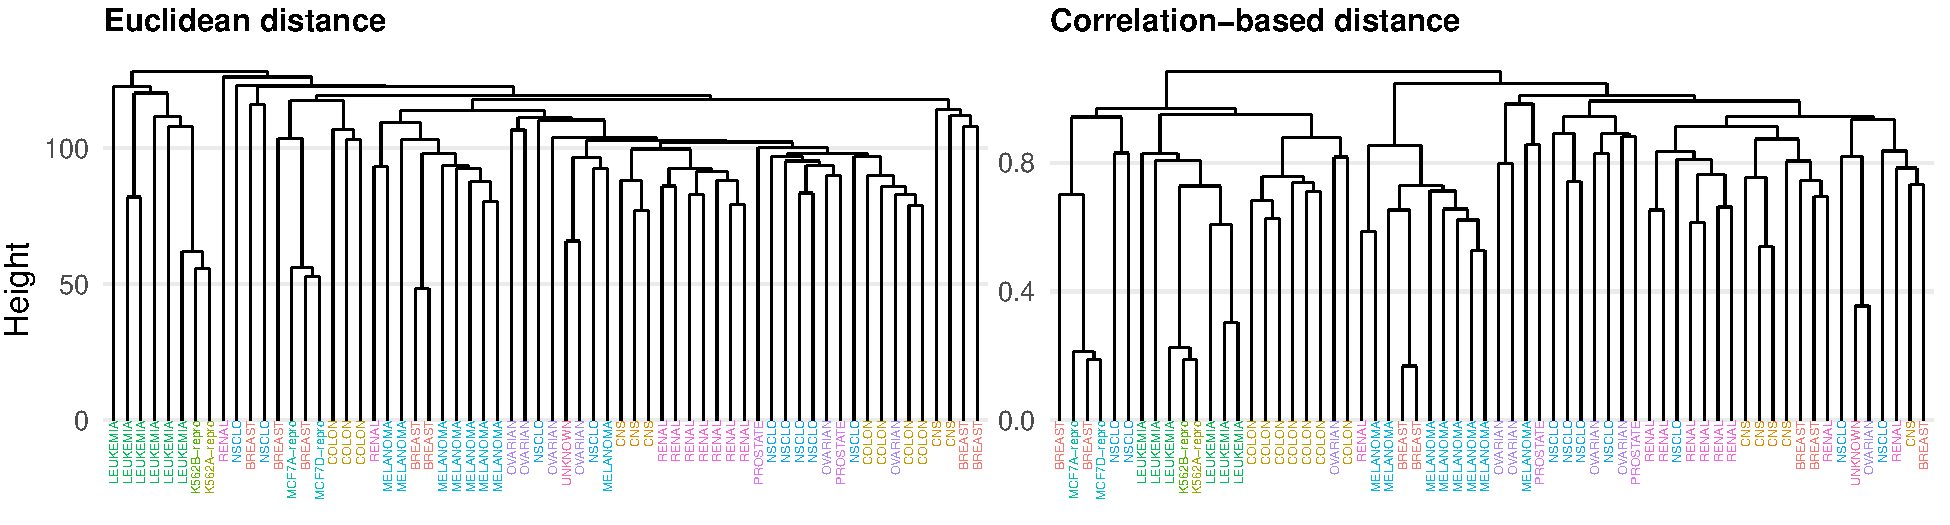
\includegraphics[width=\textwidth, height=0.5\textheight, keepaspectratio]{figures/fig_nci_dendro_distance.pdf}
    \begin{itemize}
        \item Leaves are labeled and colored by cancer type, which was not used to build the tree
        \item Average linkage with Euclidean distance (left) and correlation-based distance between cell lines (right) group the cell lines differently
    \end{itemize}
\end{frame}


% ------------------------- end of class 1 -------------------------


\section{Cluster evaluation}

\begin{frame}{Why evaluating clusters is hard}
    \begin{sitemize}
        \item Without a response there is no ground truth, and every clustering algorithm returns clusters even when the data have no cluster structure.
        \item Evaluation therefore asks several questions: how many clusters, how compact and well separated they are, whether they agree with known labels, and whether they are stable.
        \item Internal measures use only the data and the partition; external measures compare with known labels; stability checks whether the result survives small changes.
    \end{sitemize}
\end{frame}

\begin{frame}{Internal measure: within-cluster sum of squares}
    \begin{columns}[T]
        \begin{column}{0.6\textwidth}
            \begin{itemize}
                \item Total variation: $\text{TSS} = \text{WSS} + \text{BSS}$ ($\bar{\mathbf{x}}$: overall mean)
                \begin{align*}
                    \text{WSS} &= \sum_{k} \sum_{i \in C_k} \lVert \mathbf{x}^{(i)} - \bar{\mathbf{x}}_k \rVert^2 \\
                    \text{BSS} &= \sum_{k} |C_k| \, \lVert \bar{\mathbf{x}}_k - \bar{\mathbf{x}} \rVert^2
                \end{align*}
                \item $\text{BSS} / \text{TSS}$: share of variation explained by the clusters
                \item WSS always falls as $K$ grows; look for an elbow, a $K$ after which it falls much more slowly
            \end{itemize}
        \end{column}
        \begin{column}{0.38\textwidth}
            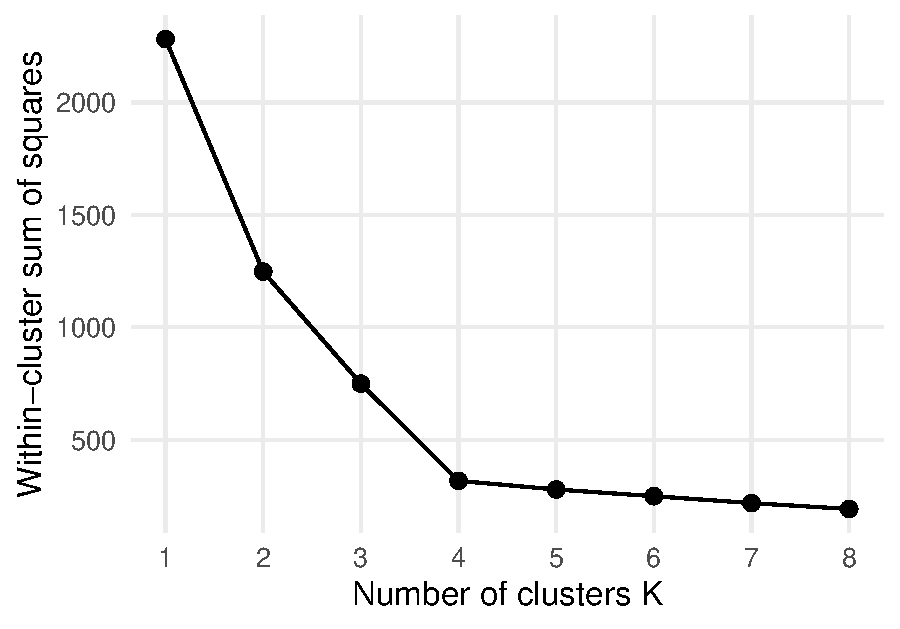
\includegraphics[width=\textwidth, height=0.45\textheight, keepaspectratio]{figures/fig_elbow.pdf}

            {\scriptsize Four-cluster simulated data. The elbow can be ambiguous.}
        \end{column}
    \end{columns}
\end{frame}

\begin{frame}{Internal measure: silhouette}
    \begin{itemize}
        \item For observation $i$ in cluster $C_k$, let $a(i)$ be its mean dissimilarity to the other members of $C_k$, and $b(i)$ the smallest mean dissimilarity to the members of any other cluster
        \[
            s(i) = \frac{b(i) - a(i)}{\max\{a(i), b(i)\}} \in [-1, 1]
        \]
        \item $s(i)$ is the silhouette width of observation $i$; near $1$: well clustered; near $0$: on the border between clusters; negative: probably in the wrong cluster
        \item The average silhouette width summarizes a partition; choose the $K$ that maximizes it
    \end{itemize}
\end{frame}

\begin{frame}{Silhouette in practice}
    \centering
    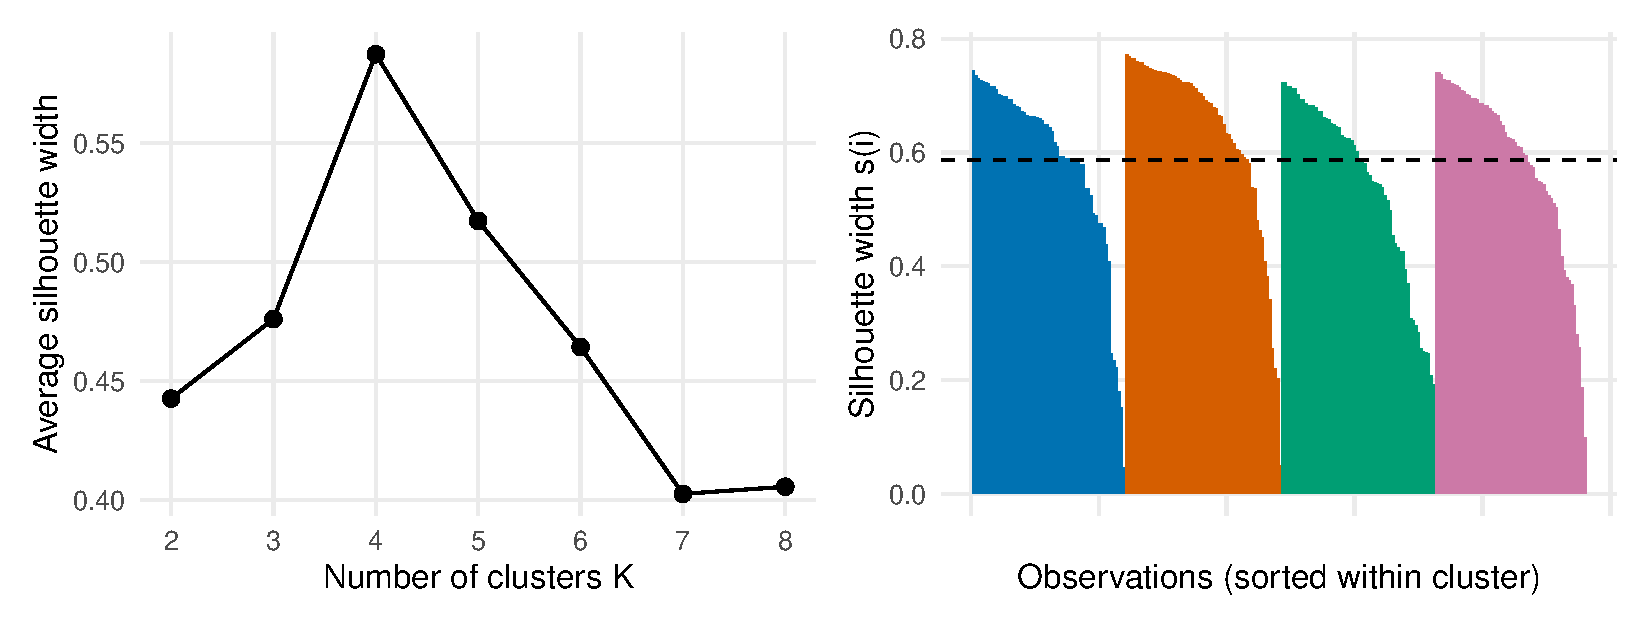
\includegraphics[width=\textwidth, height=0.5\textheight, keepaspectratio]{figures/fig_silhouette.pdf}
    \begin{itemize}
        \item Four-cluster simulated data. Left: average silhouette width against $K$; right: individual silhouette widths for the chosen $K = 4$
        \item Unlike WSS, the average silhouette does not always improve with $K$, so it can point to a best $K$
    \end{itemize}
\end{frame}

\begin{frame}{Hierarchical clustering: cophenetic correlation}
    \begin{itemize}
        \item The cophenetic distance $t_{il}$ between observations $i$ and $l$ is the height at which they first join in the dendrogram
        \item The cophenetic correlation is the correlation between the original dissimilarities and the cophenetic distances over all pairs:
        \[
            c = \operatorname{cor}\bigl( \{ d_{il} \}_{i < l}, \{ t_{il} \}_{i < l} \bigr)
        \]
        \item Close to $1$: the dendrogram represents the original dissimilarities faithfully
        \item Use it to compare linkages for the same dissimilarity% : \textttbg{cor(dist(x), cophenetic(hc))}
    \end{itemize}
\end{frame}

\begin{frame}{External measure: Rand index and adjusted Rand index}
    \begin{itemize}
        \item When reference labels exist, compare the partition $U$ with the labels $V$ through pairs of observations
        \item Rand index: the fraction of pairs on which $U$ and $V$ agree, i.e. both place the pair together or both place it apart
        \item The adjusted Rand index corrects for agreement by chance. With $n_{ab}$ the number of observations in cluster $a$ of $U$ and class $b$ of $V$, and $n_{a\cdot}$, $n_{\cdot b}$ the row and column totals,
        \[
            \text{ARI} = \frac{\sum_{a,b} \binom{n_{ab}}{2} - t}{\frac{1}{2} \Bigl( \sum_{a} \binom{n_{a\cdot}}{2} + \sum_{b} \binom{n_{\cdot b}}{2} \Bigr) - t}, \quad t = \frac{\sum_{a} \binom{n_{a\cdot}}{2} \sum_{b} \binom{n_{\cdot b}}{2}}{\binom{n}{2}}
        \]
        \item ARI $= 1$ for identical partitions and about $0$ for random labeling (it can be negative)
    \end{itemize}
\end{frame}

\begin{frame}{NCI60: agreement with cancer type}
    \centering
    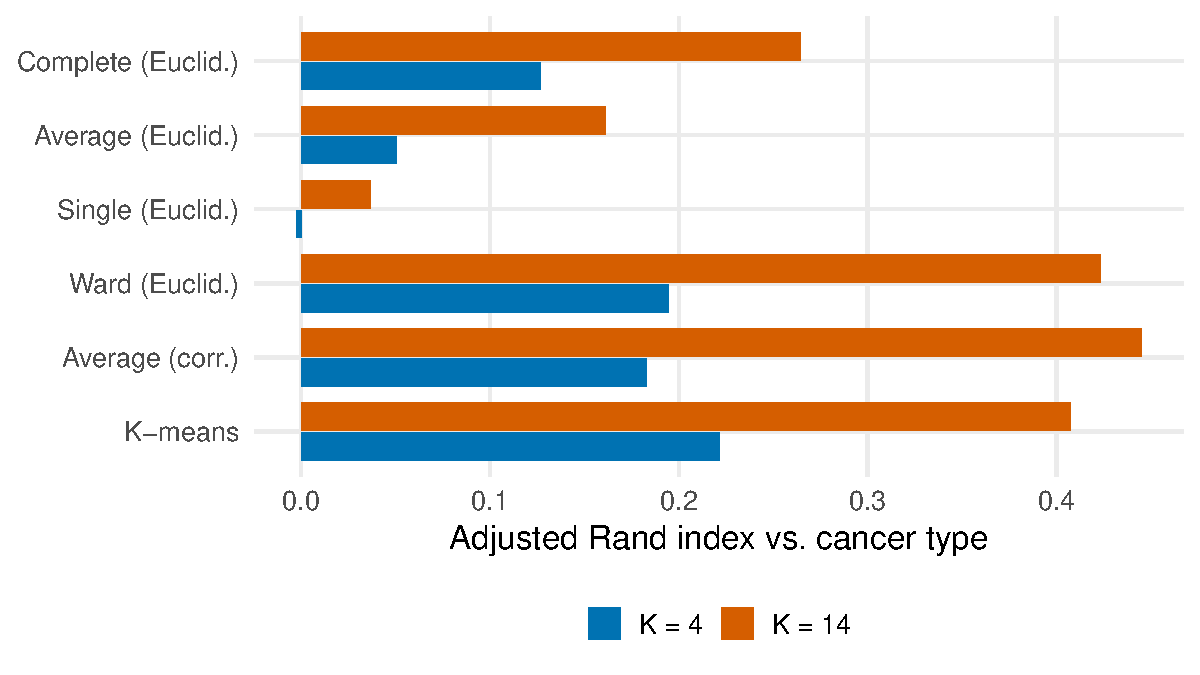
\includegraphics[width=\textwidth, height=0.42\textheight, keepaspectratio]{figures/fig_nci_ari.pdf}
    \begin{itemize}
        \item ARI between each clustering and the 14 cancer types, for $K = 4$ and $K = 14$ clusters
        \item Labels are not necessarily the true clusters: a low ARI may reflect a mismatch between the labels and the gene expression, not a bad clustering
    \end{itemize}
\end{frame}

\begin{frame}{Stability and robustness}
    \begin{itemize}
        \item Clustering can be sensitive: removing a few observations or changing a setting may change the clusters
        \item Re-cluster on subsamples or bootstrap samples and check whether the same groups reappear% (\textttbg{fpc::clusterboot})
        \item Vary the choices: $K$, standardization, dissimilarity, linkage, and random starts
        \item Report conclusions that hold across reasonable choices, and treat the rest as uncertain
    \end{itemize}
\end{frame}

\begin{frame}{Evaluation tools: summary}
    \centering
    \footnotesize
    \begin{tabular}{@{}l l p{5.6cm}@{}}
        \toprule
        Tool & Needs labels? & Answers \\
        \midrule
        WSS and elbow & no & how much variation $K$ clusters explain; choosing $K$ \\
        Silhouette & no & how well separated and compact; choosing $K$ \\
        Cophenetic correlation & no & how well a dendrogram preserves the dissimilarities \\
        Adjusted Rand index & yes & agreement with a reference partition \\
        Stability (resampling) & no & whether the clusters are reproducible \\
        \bottomrule
    \end{tabular}
\end{frame}


\section{Cluster interpretation}

\begin{frame}{Profiling the clusters}
    \begin{columns}[T]
        \begin{column}{0.5\textwidth}
            \begin{itemize}
                \item Report each cluster's size $|C_k|$ and centroid $\bar{\mathbf{x}}_k$ in original units
                \item Compare clusters on a common scale with standardized means $(\bar{x}_{kj} - \bar{x}_j) / s_j$; $\bar{x}_{kj}$ is the mean of variable $j$ in cluster $k$
                \item Variable-by-variable tests (ANOVA) are descriptive only: the clusters were chosen to differ, so $p$-values are not valid
            \end{itemize}
        \end{column}
        \begin{column}{0.48\textwidth}
            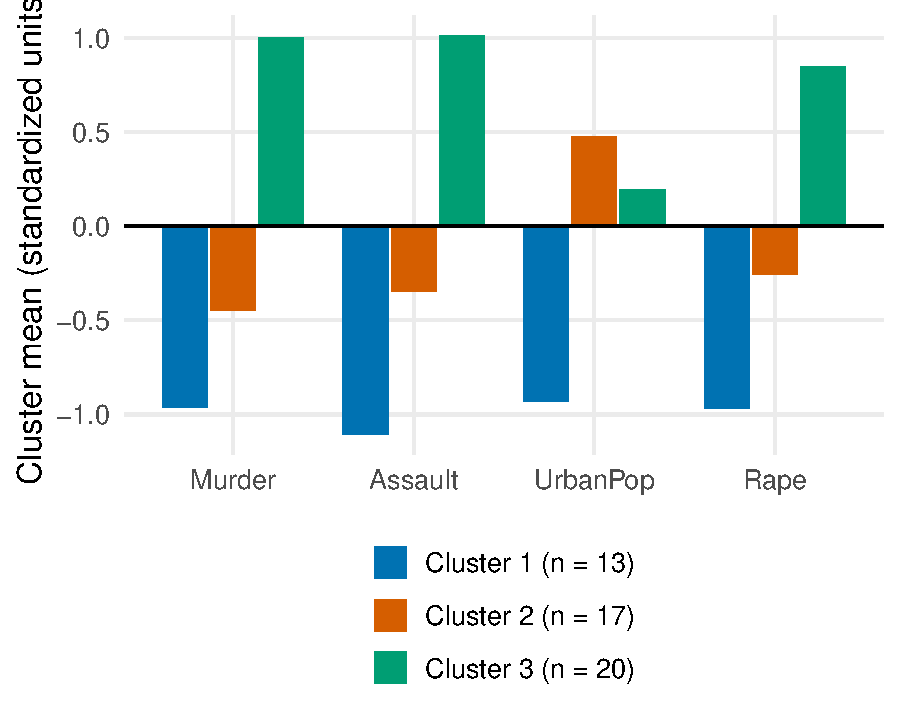
\includegraphics[width=\textwidth, height=0.6\textheight, keepaspectratio]{figures/fig_usarrests_profile.pdf}

            {\scriptsize USArrests, K-means with $K = 3$}
        \end{column}
    \end{columns}
\end{frame}

\begin{frame}{Visualizing clusters: pairs plot}
    \centering
    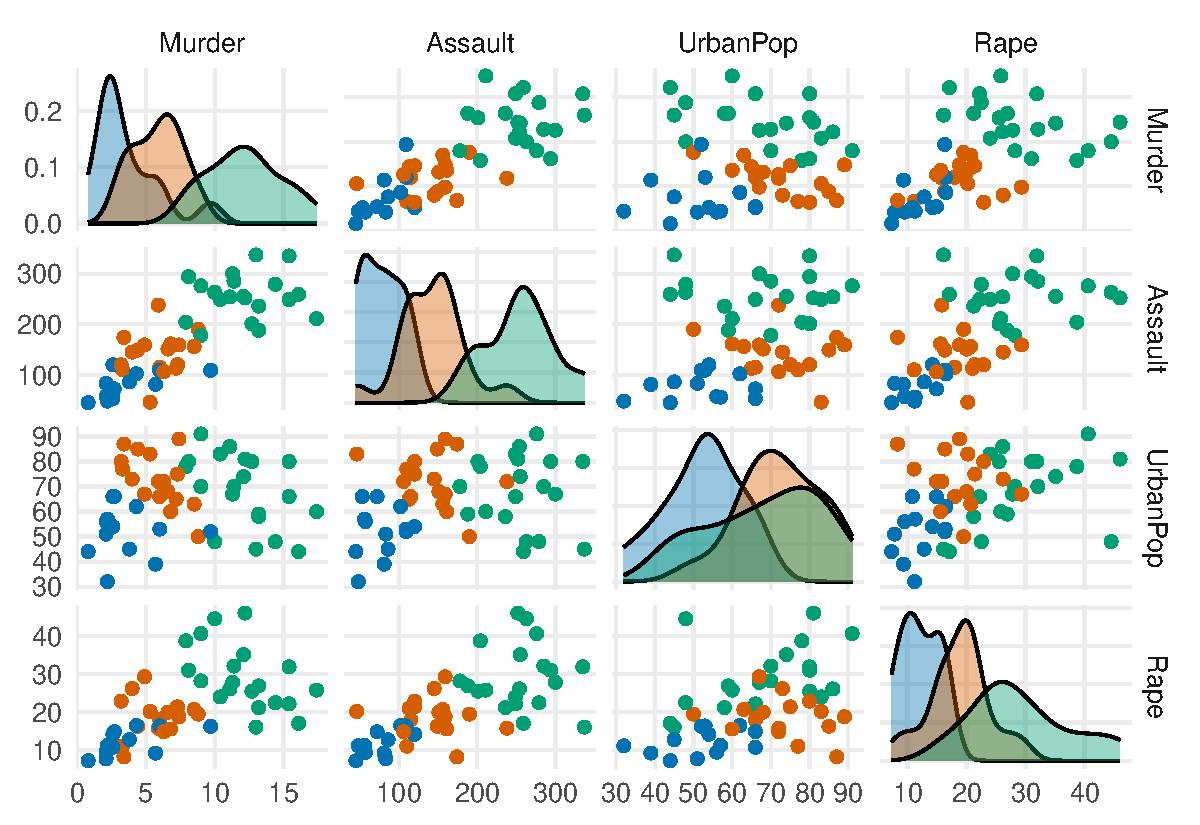
\includegraphics[width=\textwidth, height=0.68\textheight, keepaspectratio]{figures/fig_usarrests_pairs.pdf}
    \begin{itemize}
        \item Every pair of the original variables, colored by cluster: shows directly which variables separate which clusters
    \end{itemize}
\end{frame}

\begin{frame}{Interpreting and reporting clusters}
    \begin{sitemize}
        \item Name clusters from their profiles, but remember that a cluster is a description of this sample under one set of choices, not a discovered ground truth.
        \item Report the dissimilarity, standardization, algorithm, $K$, number of starts, and the evidence from evaluation and stability.
        \item Check the clusters with subject-matter knowledge or new data; do not use the same variables to test whether the clusters differ.
        \item Cluster labels can be used downstream, for example as a feature in a supervised model.
    \end{sitemize}
\end{frame}


\begin{frame}{Summary}
    \begin{itemize}
        \item Clustering partitions unlabeled observations; the result depends on the dissimilarity, scaling, algorithm and $K$
        \item Standardize unless variables share a meaningful scale; correlation distance for profile shape, Gower for mixed data
        \item K-means minimizes within-cluster sum of squares with Lloyd iterations, so use many starts; hierarchical clustering gives a dendrogram for any $K$, and the linkage matters
        \item Evaluate with elbow and silhouette for $K$, cophenetic correlation for dendrograms, ARI when labels exist, and stability always
        \item Interpret with cluster profiles and visualizations; reading: ISLP Chapter 12, Section 12.4
    \end{itemize}
\end{frame}
